\section{Planning and execution in the \texttt{T-REX} architecture}
\label{sec:arch}

\subsection{The T-REX architecture}
\label{sec:arch:trex}

% {\em\tiny This section introduces shortly T-REX architecture but move
%   quickly the focus on a single reactor and gross concepts on the
%   architecture:
%   \begin{itemize}
%   \item For t-trex the whole decision and control problem is reduced
%     around the state variables (or timeline construct). 
%   \item This reduce the execution tracking problem for each reactor on a state
%     identification problem (deduce internal state from the external
%     state), and the control problem to goal posting which will trigger
%     deliberation on the owner of the corresponding timeline. 
%   \item the architecture itself see each reactor as a black box and
%     therefore each reactor can implement its own mechanism in order to
%     resolve both synchronization and deliberation. Still we provide a
%     reactor based on the europa framework that leverage the automated
%     planning capabilities in order to do model based planning and
%     execution with a rich representation of resources and time.
%   \end{itemize}}
 
The T-REX architecture was designed with the objective to bring 
planning closer to the low-level control of the vehicle while
maintaining its reactivity. Indeed, in most of the architecture where
task planning is embedded, this task remains at a failry high level of
abstraction as the complexity of this task would otherwise impede the
system reactiveness. As a result the planning problem managed {\em in
  situ} remains fairly detached from low-level control and most of the 
reactive adaptation which in contrast is managed by specialized 
component that relies on different representations for modeling 
the local behavior they control or even do not have any explicit 
formal model of this behavior. Taking cues from the IDEA 
architecture \cite{mus02}, we designed a core framework that provides a
formal basis \cite{Py:2010ti} on the way each of the sub-component --
called reactors -- of our agent can interact by exchanging only
information through {\em state variables} by ensuring that state 
information can propagate through all the reactors ensuring a
consistent view of the present state of the world at every single tick
trough a bottom-up {\em synchronization} flow and collaboration for
future state evolution by timely exchanges of goals on {\em state
  variables}. This exchange does not impose to any reactor to be aware
of the reactors it is connected to but only focus on the state
variables it relies on (called {\em external}) and the state
variables it manages and maintains (called {\em internal}). 

Take for example the T-REX agent instance we use in our AUV
(Fig. \ref{fig:agent}). In this architecture all the reactors
(symbolized by colored boxes) do not have explicit connection from one
to another but instead rely on a publish/subscribe model on state
variables. For Example the \textsf{Pilot} reactor needs the {\em
  externally} managed state informations from \textsf{Sensor\_Data} 
and \textsf{Nav\_cmd} states variables in order to maintain {\em
  internally} the state variables \textsf{Waypoint} and
\textsf{Nav\_policy}. This relation applies in two way :
\begin{itemize}
\item In order to identify its current {\em internal} state values
  this reactor needs to know the current {\em external} state
  information it relies on. In this case the current \textsf{Waypoint}
  the vehicle is heading to can be extracted for example from the
  current \textsf{Nav\_cmd} executed.
\item The future objectives a reactor has on its future \textsf{Internal}
  state will probably imply sub-objectives to be reported to the
  owner of its {\em external} depending on their current values. Again
  if this reactor wants to go ato a specific \textsf{Waypoint} --
  depending on its current position provided by \textsf{Sensor\_Data}
  it can identify a sequence of \textsf{Nav\_cmd} that should
  eventually help him reach this location.
\end{itemize}

\begin{figure}[!htb]
 \centering
 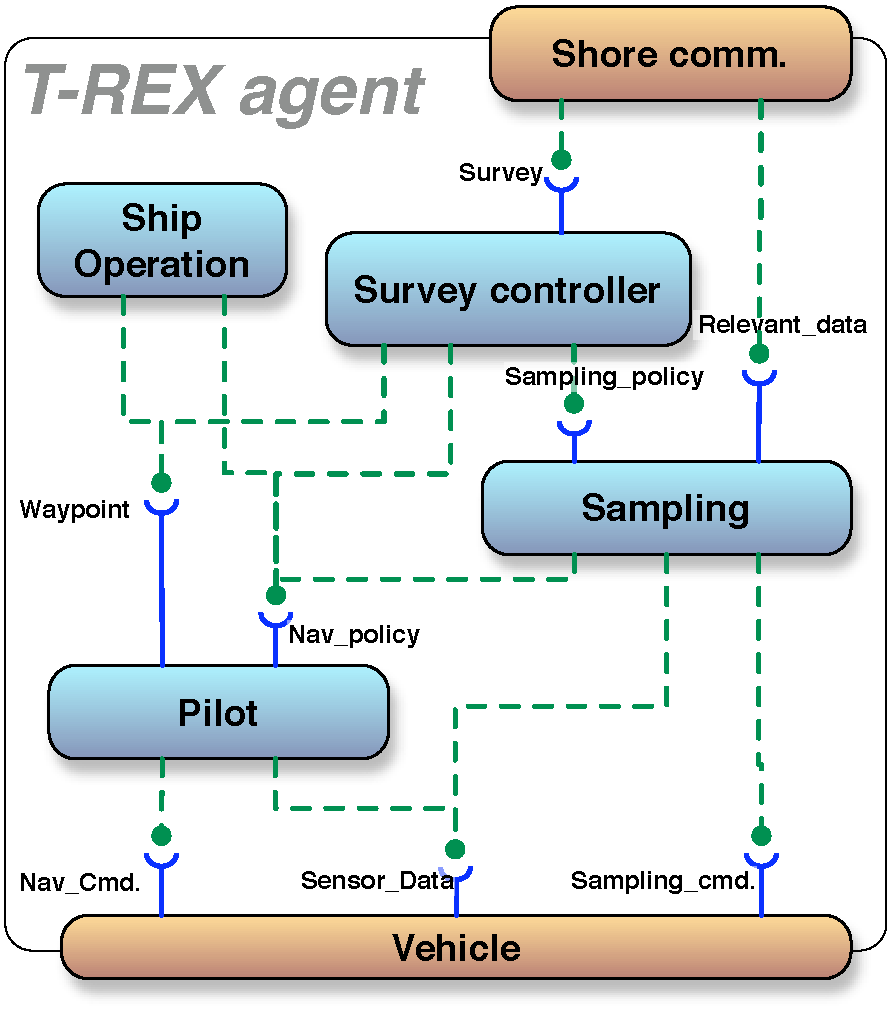
\includegraphics[scale=0.45]{figs/AUV-agent.pdf}
 \caption{\small A \texttt{T-REX} agent is composed of multiple
   reactors or control loops (rounded boxes) which are connected
   through state variables provided by one reactor ({\color{blue}blue}
   solid line) with multiple possible clients ({\color{green}green}
   dashed lines)}
  \label{fig:agent}
\end{figure}

Overal T-REX architecture helps to abstract to the reactor interaction
to only state variables. Each reactor is practically ignoring where
its {\em external} state information is managed as long as this
information is available and properly maintained so they can properly 
manage their own {\em internal} state information which in turn may be
used by other reactors. Such formalism also constrain reactors
interaction to state information exchanges which are two folds:
\begin{itemize}
\item {\em Observation on the current state values}: This information
  propagates up in the reactor graph at the synchronization phase 
  and occur at the beginning of every time steps (called
  ticks). During this phase the agent provides to each reactor 
  updates on their {\em external} state variables for this tick and
  ask them to compute their {\em internal} state variables values for
  this same tick. By doing so we propagate a consistent view of that
  state of the world throughout all the reactors as time advance.
\item {\em Goals request on future state}: This information propagates
  down in the reactor graph. It reflects that, in order to satisfy own
  of its {\em internal} objectives, a reactor may have a plan that
  rely on future values of one of its {\em external} state. When such
  a plan is identified we ensure that this part of the plan is given
  as a goal to the owner of the given {\em external(s)} state variable(s). 
\end{itemize}

The overal execution cycle of the agent is emerging through these
interaction and the processing that occurs in each reactors in order
to process them. New observation occurring at every tick inform each
reactor of the current state of the world and impose them to identify
how it impact their state (and potentially what they planned for the
future). Goals they receive will trigger in the reactor the need to
identify a strategy (or plan) that will allow them to reach these new
states knowing their current state deduced from synchronization.When
such a plan has been identified, the {\em external}  part is then
dispatched to other reactors that can do the same. This flow and focus
around state and goals is perfectly fitting with automated planning
and even more so to the Europa framework. As an illustration, in 
 Fig. \ref{fig:agent}, only \textsf{Shore comm.} and \textsf{Vehicle}
 reactors are specialized C++ code (acting as interface to external
 programs). All the other reactors are based on the europa framework
 differentiated only by the domain model they manipulate and som
 heuristic configuration parameters. In the following sections we are
 going to focus specifically ion this kind of reactor to illustrate
 how  a formal planning framework can be used in our architecture to
 both track state evolutions and plan for future objectives while
 remaining efficient enough to do these tasks in a real-time control 
loop.

\subsection{The Europa deliberative reactor}
\label{sec:arch:europa}

In T-REX architecture reactors have two core functions;
synchronization where the main focus is to track and refine the
evolution of the state of the world at any single tick, and
deliberation which focus on providing a plan to the agent in order to
complete the reactor {\em Internal} goals. These two processes are
intertwined in the sense that one influences the outcome of the
other. They are represented as two europa solvers modifying the same
plan database and for which the execution is managed by the T-REX 
framework as time advance during the execution of the system:
\begin{enumerate}
\item The synchronization solver is a specialized europa solver that
  will integrate in the plan new information about the evolution of
  the External state variable and ensure that the reactor propagate
  these in order to both identify its current state and inform
  other reactors of any state change on its internal timelines. This
  solver is summoned at the beginning of every single tick.
\item The deliberation solver is managing the deliberation process of
  the reactor in order to produce a new plan or alter its current plan
  as new goals are given to the reactor or the synchronization solver
  identifying a conflict between the current state of the world and
  the expectations of the previous plan. This process can  span other
  multiple tick and therefore can be interrupted at any single tick in
  order for the synchronization solver to do its task.
\end{enumerate}

While synchronization is assumed to be fast enough that it can be
resolved in less than a tick. Deliberation on the other hand can take
several ticks reflecting that automated planning can take time
depending on how far in the future the planner is looking ahead and
the complexity of the model. T-REX architecture, and more specifically
the europa based reactor in our case, takes this into account by
considering synchronization and deliberation as two concurrent tasks
with their own timing requirements and priority. 
While the two processes are separate, they share the same plan
internal to a reactor and therefore at every synchronization cycle the
planning process is informed of the new world state and its impact on
the plan. Conversely, when the planning process eventually finds a
solution, synchronization is informed about generating the planned
state values on the {\em external} state variables. This {\em
  external} plan defines the set of {\em goals} for this state
variable managed by another {\em reactor}. Fig. \ref{fig:tick-exec}
shows a conceptual view of these two tasks.


\begin{figure}[!htbp]
  \centering
  \vskip-1pc
  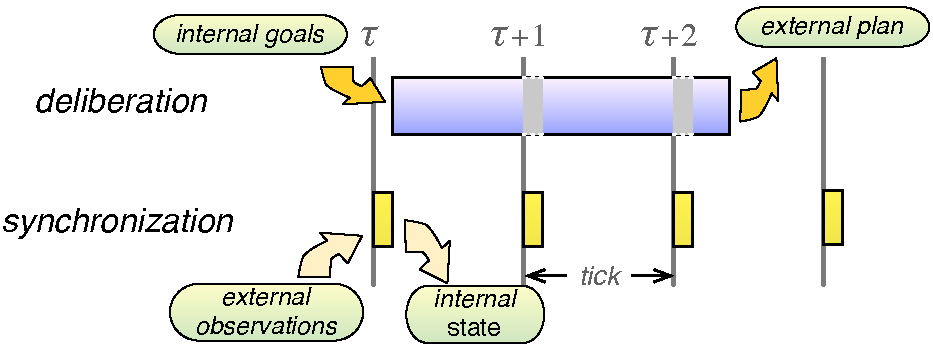
\includegraphics[width=0.55\columnwidth]{figs/tick-cycle}
  \caption{\small \texttt{T-REX} reactor execution cycle: {\em
      Deliberation} is interrupted by {\em synchronization} at the
    beginning of every {\em tick} allowing integration of state
    information.}
  \label{fig:tick-exec}
  \vskip-0.8pc
\end{figure}


In  this section we present how both processes are implemented using
the europa framework. We first present each of them independently by
looking to their specific focus. We then develop how both processes
are not only interleaved (as deliberation can take several tick while
synchronization eneds to happen at every single tick) but also discuss
on how each of these is impacting the other and how this intertwining 
of the two result on an emergent behavior of the reactor by allowing
the system to efficiently adapts its plan that can then be dispatched
as objectives for the reactors it depends on in a seamless flow. 




{\em fpy: I still wonder whether I should start with planning assuming
  first that the initial state is known and then develop
  synchronization and how it ties state information in to the plan or
  the other way around as it is now}

\subsubsection{Synchronization identify internal state evolution}
\label{sec:arch:synch}


For the sake of simplicity we introduce first how a reactor can track
and identify its state in the context where it does not have any
compelling need to deliberate. Assume here that we have a reactor that
have no future goal. {\em Need to develop the reason why it is a
  necessity: primarily to provide its internal state to whoever
  observe it but als simply to ensure that its current representation
  of the world is up to date and still consistent}

In the europa based reactor we introduce this requirement as a new
type of flaw for the europa framework. This flaw enforces at the
reactor to identify fully its internal state for the current
tick. By using this new flaw we can describe the synchronization
process as this general sequence :
\begin{enumerate}
\item Integrate the external state as provided by the owner of each
  external timeline into the plan database.
\item Propagate this information in the plan database following the
  model $\mathcal{M}$ of this reactor.
\item Resolve the current state value of each internal timelines.
\end{enumerate}

\begin{figure}[!htbp]
  \centering
  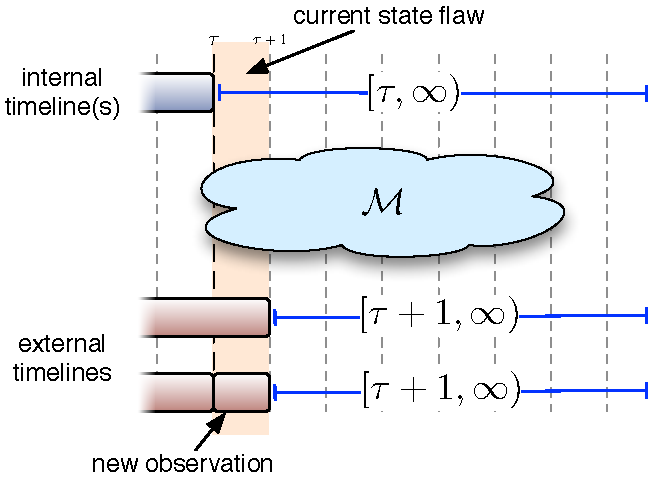
\includegraphics[width=0.5\columnwidth]{figs/synch-relation}
  \caption{Ilustration of the synchronization flaws in a reactor. The
    reactor receive new observations when they are produced by the
    owner(s) of its internal timelines. The line after the last token
    of each timeline represent the domain of possible values for the
    end of this token. At every tick $\tau$ the reactor needs to
    integrate the {\em External} state information it received and --
    based on its model $\mathcal{M}$ -- resolve its {\em Internal}
    state that will then be provided by the architecture to other
    reactors using these state variables.}
  \label{fig:synch:flaw}
\end{figure}

The resolution of internal state flaw can be resolved using one of the
following choices which are evaluated in the given order:
\begin{enumerate}
\item Extend the previous state value to end after this tick (ie
  restrict its end time to $[\tau+1, \infty)$). 
\item Start the next active token in the timeline and
  attempt to start it now (ie restrict its start time to the single
  value $\tau$).
\item Create and insert a new token in this timeline that will start
  at the current tick $\tau$ (attempt this for each possible token
  type for this timeline if necessary). 
\end{enumerate}

All of these choices are evaluated sequentially until a consistent
solution with no more flaw for this tick is identified. In order to do
so we need to make the assumption that the current state value of an
internal timeline do not depend on the future or more accurately
that any choices made during this synchronization will not lead to a
future inconsistency (meaning no possible solution) for a future
synchronization. Such assumption deeply impact the set of possible
domains one the reactor can support while remaining complete. Take for
example the following model rule where {\tt Vehicle} is {\em Internal}
and {\tt Command} is {\em External} to the reactor.
\begin{verbatim}
Vehicle::Dive {
  contains(Command.Descend descend);
  descend.start = start + 2;
}
\end{verbatim}

Such model present the issue that the reactor needs at one point to
take the decision to start the token {\tt Vehicle.Dive} and by doing
so it assumes that in {\em exactly} 2 ticks in the future the {\tt
  Command} timeline will change its state to {\tt Command.Descend}. If
this observation does not occur at the given time this implies that
the reactor estimation was wrong leading him to an inconsistent view
of the world. Conversely the reactor can decide to not switch this
timeline to the {\tt Vehicle.Dive} state and observe 2 ticks in the
future that the {\tt Command.Descend} state value. In this case it
would have missed the opportunity to set its {\tt Vehicle} state to
the correct value which may similarly lead (depending on the rest of
the model) to a similar inconsistency it won't be able to resolve (as
TREX enforces that  the past is monotonic).

While this limitation of the system is important to take into account,
it is also important to note that the model snippet we gave here --
while formally acceptable in the general planning problem -- is also
illustrating a bad design for execution in a situated agent. Indeed,
in this model we are tying the current decision to a future outcome
that is {\em External} to the reactor and therefore not necessarily
controllable by this reactor. Therefore we are entailing a part of the
future to past decisions which can lead the system to a dead-end
situation where the model cannot find a correct solution that both do
not conflict with what we claimed in the past and still allow the
planner to find its current {\em Internal} state.


\subsubsection{Deliberation : planning for future state evolution}
\label{sec:arch:plan}




\subsubsection{Intertwining synchronization and execution }
\label{sec:arch:intertwine}




% Gives a high-level overview of T-REX, the general design principles and how
% these principles aid in software engineering. Show T-REX block diagram.



%%% Local Variables: 
%%% mode: latex
%%% TeX-master: "setobook"
%%% End: 
